
\setlength{\tabcolsep}{10pt}
\begin{table*}
\centering
\begin{tabular}{clccc}
\hline
   \multicolumn{2}{l}{independent variables} &min&max&Nbins\\
\hline
   $\tau_{a}$ & Mean temporal separation between consecutive awakenings & 4000 y & 200000 y & 50\\ 
   $\tau_{s}$ & Mean lifetime of a MPL                                 & 10000 y & 500000 y& 50\\ 
   D$_{max}$ & Maximum reach of a message  &  \multicolumn{3}{l}{500, 1000, 10000, 20000, 40000, 80000 lyr}  \\
\hline
   \multicolumn{4}{l}{fixed variables and assumptions} &value \\
\hline
   & statistical properties of all MPLs &equally distributed&&\\
   & Point process for the distribution in time & homogeneous &&\\
   f$_s$ & The scan of the sky & fully efficient&&1\\
   f$_p$ & panspermia or colonization &absent&&0\\
   & shape of the Galactic Habitable Zone & 2--dimensional ring &&\\
   R$_{SFC}$   & Inner radius of the GHZ     &&&20000 ly\\
   R$_{SLC}$   & Outer radius of the GHZ     &&&60000 ly\\
   t$_{max}$ & Time span of the simulation  &&&1.e6 y\\
\hline
   \multicolumn{5}{l}{discrete events}\\
\hline
   A & Awakening: a civilization starts a SETI program  &&&\\
   B & Blackout: the end of the communication chanel stops &&&\\
   C & Contact: a new causal contact is produced &&&\\
   D & Doomsday: a civilization ends its communication capabilities&&&\\
\hline

\hline
\end{tabular}
\caption{Definition of independent variables and adopted values for 
   fixed paramenters 
   that are part of the simulation.  Variable parameters define the
   spatial and temporal structure
   of the process and the maximum reach of the messages.}
\label{T_simu_hypotheses}
\end{table*}

 


\begin{figure*} % 2D color plot
   \centering
   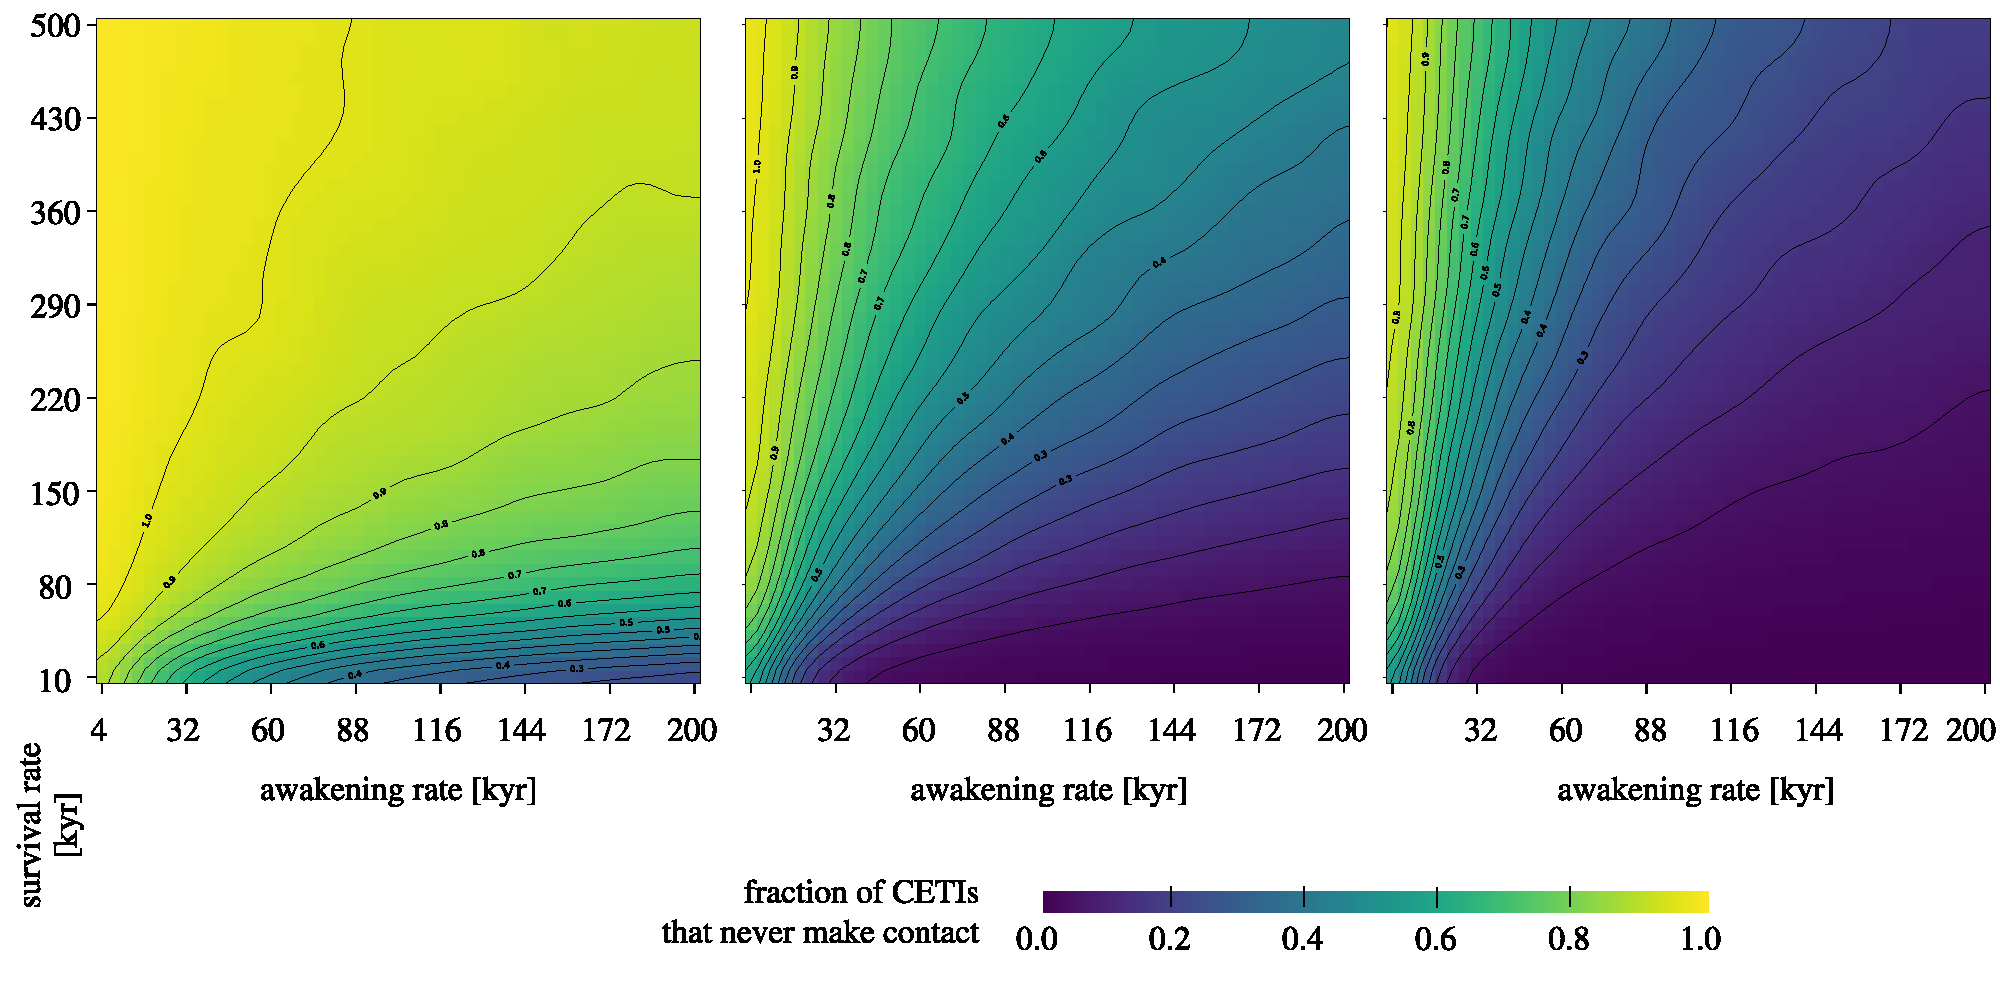
\includegraphics[width=\textwidth]{matrix_1.pdf}
   \usecaption{F_never_contact}
   \label{F_never_contact}
\end{figure*}
 
\begin{figure*} % 2D color plot
   \centering
   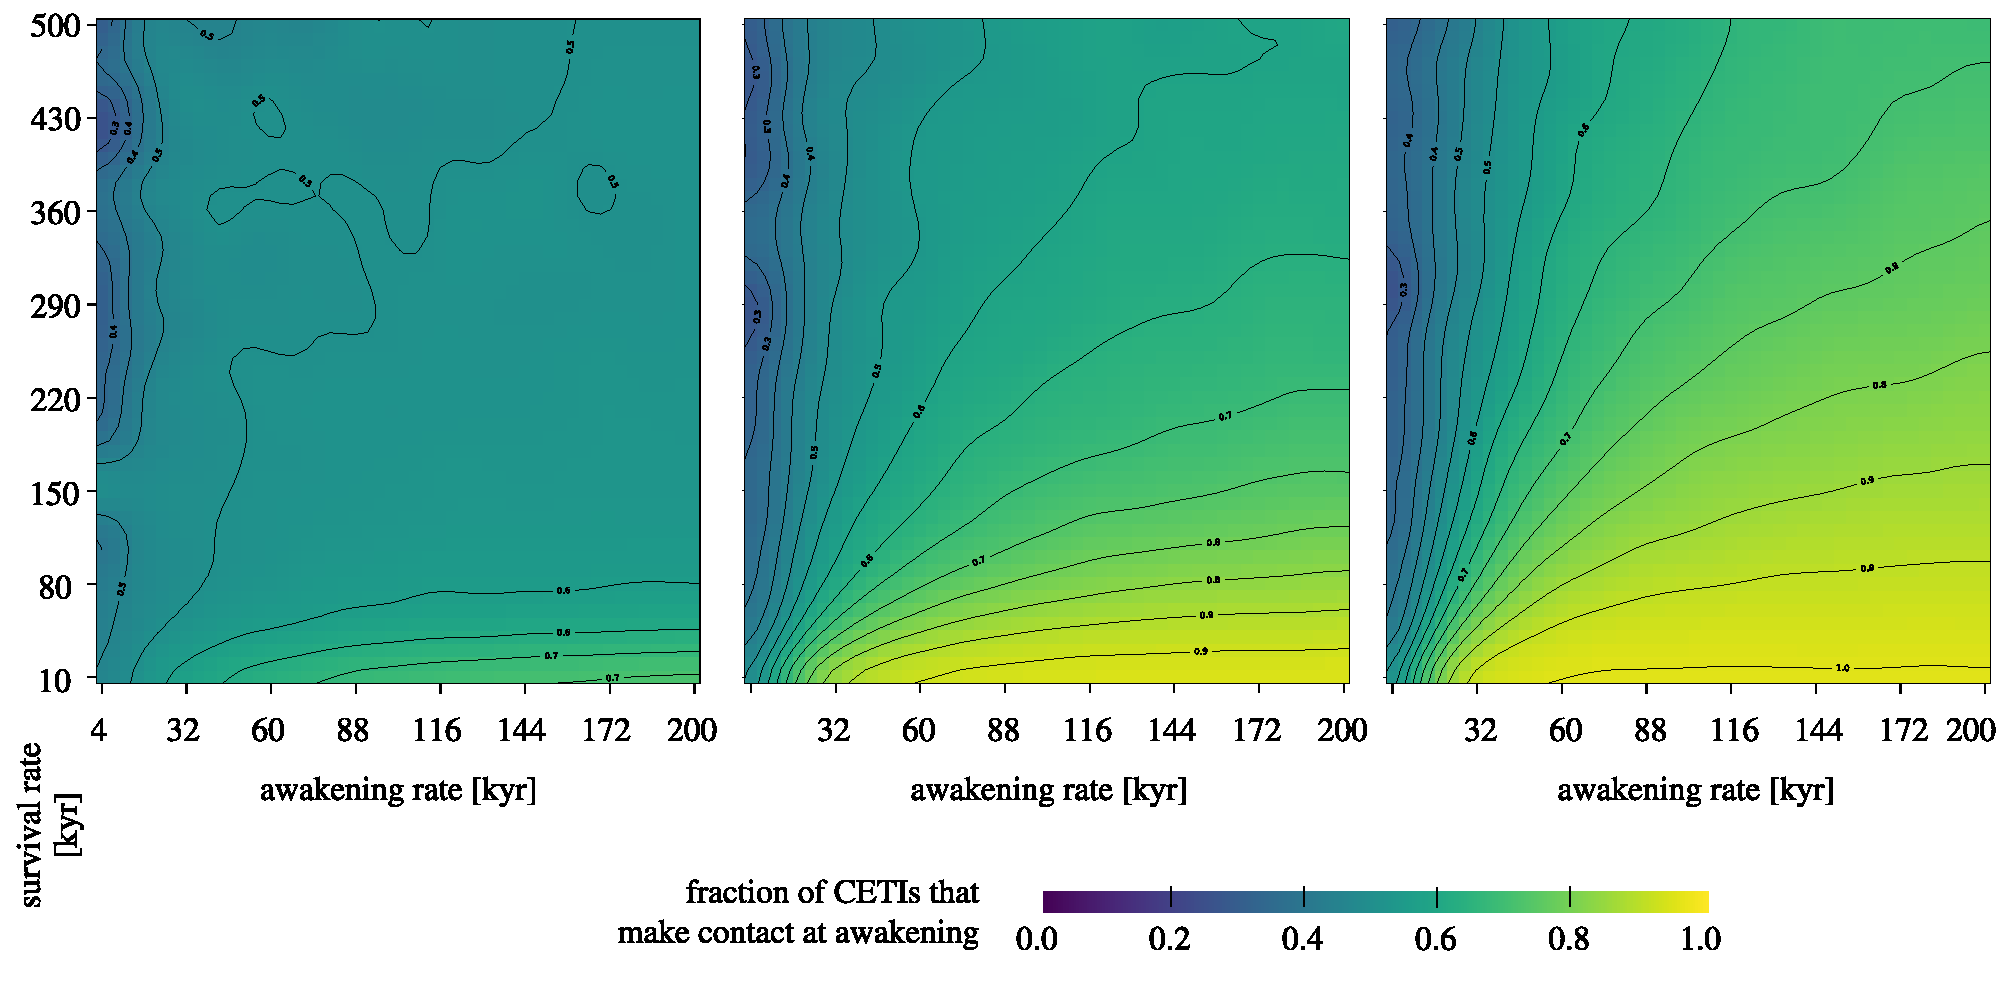
\includegraphics[width=\textwidth]{matrix_2.pdf}
   \usecaption{F_C_at_A}
   \label{F_C_at_A}
\end{figure*}
 
\begin{figure}
   \centering
   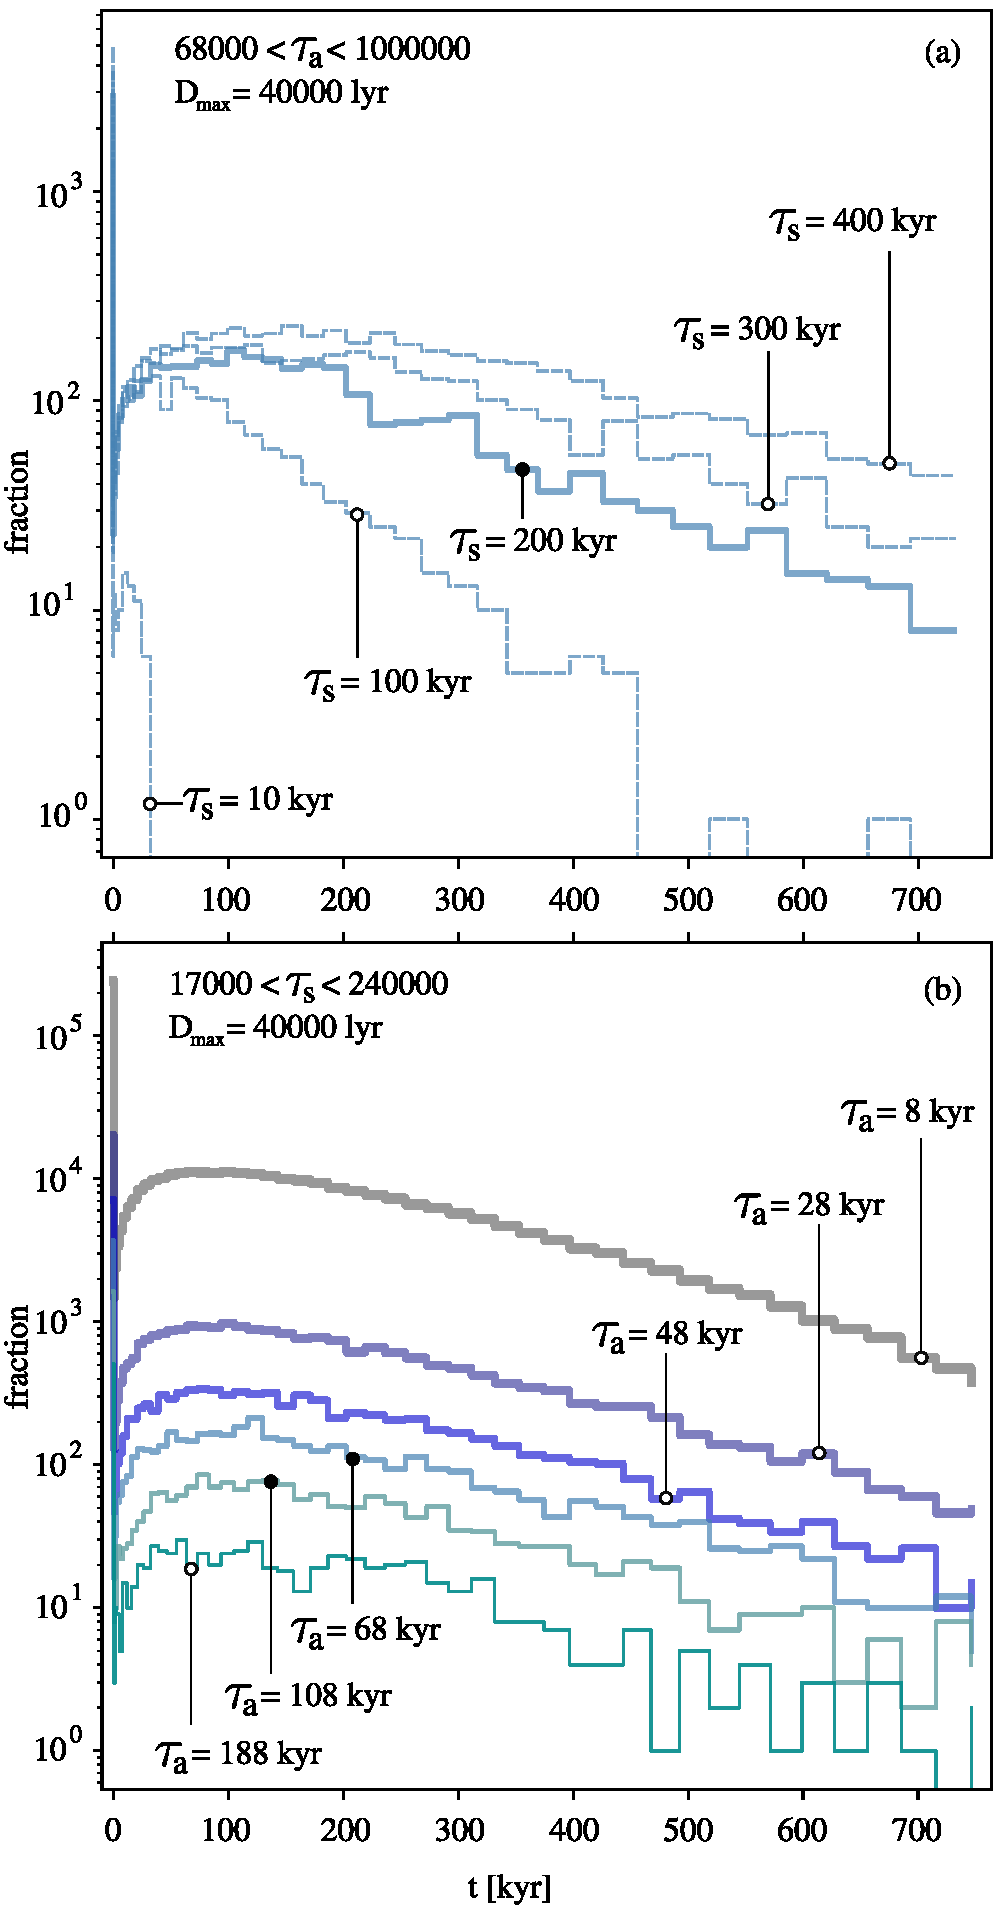
\includegraphics[width=0.5\textwidth]{waiting_s+a_dif_ylog.pdf}
   \usecaption{F_waiting_for_1C}
   \label{F_waiting_for_1C}
\end{figure}


  

 

%%% S E C T I O N - - - - - - - - - - - - - - - - - - - - - - -
\section{Results: exploring the parameter space}\label{S_results}
%{{{

We implemented the simulation of a regular grid of models varying over
the hypothesis space, which covers 15000 different models.
%
For each model, we simulated 50 realizations with different random
seeds, in order to perform a MonteCarlo estimation of the variance.
%
The parameters for the temporal aspects of the simulation (the mean
waiting time for the next awakening $\tau_a$ and the mean lifetime
$\tau_s$) cover the ranges 4000-200000 yr and 10000-500000 yr,
respectively, with a regular partition of 50 values for each
parameter.
%
For the D$_{max}$ parameter, we chose the values 500, 1000, 10000,
20000, 40000 and 80000 lyr.
%
This setup makes a total of 750000 simulations, each covering a time
range of one million years.
%
In Table \ref{T_simu_hypotheses} we show the set of fixed parameters
and hipotheses that define the runs of the simulations, along with the
list of variable parameters and the range of their values that have
been explored in the numerical experiments.


As a product of the simulations, several quantities can be obtained.
%
Some quantities are directly derived from the discrete events, namely,
the ID of emitting and receiving MPLs, the position in the galaxy, and
the times of each of the events that are relevant to keep track of the
number of MPLs (time of awakening and time of doomsday) and of the
number of contacts (the times of contacts and the times of blackouts).
%
We can also derive the additional quantities that represent the
properties of the MPLs, for example the total time elapsed between the
awakening and the doomsday of each MPL.
%
The time span of a MPL listening another or being listened by another
can also be easily derived from the results of a realization.
%
This way we can also compute the distribution in the galaxy of MPLs
that reach contact and the waiting time until the first contact or the
waiting time until the next contact.
%
Regarding the properties of the population of MPLs and its evolution,
the simulation yields the fraction of awaken time a MPL is listening
at least another MPL (i.e., in their causal cone), the age of
contacted MPLs at first contact, the distribution of time to wait
until next contact, the fraction of MPLs where the first contact is
given at the awakening, the distribution of the number of contacts for
each MPL, the distribution of the number of contacts as a function of
MPL age, the number of contacts as a function of time in the galaxy,
the rate of MPLs that succeed in contact, and the distribution of
distances between contacted MPLs.
%
Another usefull derived quantity is the duration of two-way
communication channels or the fraction of contacts that admit a
response.
% 
It is also possible to analyze the relations between the distance to
MPL vs. the time of double communication, the distance to MPL vs. the
age of contacted MPL, the age of a MPL and the maximum number of
contacted MPLs before doomsday, or the lifespan of a MPL vs. the
maximum number of contacts.
%
In addition, all these quantities can be analyzed as a function of the
simulation parameters.
%
We chose eight models that are on fairly oposed regions of the
explored parameter space, and cover short/long lifetimes, short/long
waiting times for the next MPL to appear in the Galaxy and short/large
range reach of the signal, including all possible combinations.
%
The details of each model are summarized in the
Table~\ref{T_selected_models}.



In Fig.~\ref{F_number_of_contacts} we show the Empirical cumulative
distributions of the number contacts for MPLs in four different
samples (M5, M6, M7, M8) with long range signal reach
(D$_{max}$=10000). 
%
The lifetime is more determinant than the awakening rate in increasing
the number of contacts.
%
As expected, of the four samples, the sample M7, which corresponds to
a dense awakening in the timeline and a long lifetime, is the model
that maximizes the number of contacts, reaching a maximum of order 100
contacts for a single MPL.
%
This is considerable larger than any model with a shorter lifetime,
which produce a number of contacts of at most the order of ten
contacts per MPL.
%
A couple of comments are worth to mention about this plot.
%
First, it has a logarithmic scale on the x-axis, and second it is the
cumulative, not differential, empirical distribution.
 

In what follows, we focus on the analysis of the duration of contacts
(Sec.~\ref{SS_multiplicity}), the waiting time for the first contact
(Sec.~\ref{SS_waiting}) and the
variations of contact posibilities as a function of the position of
the MPL in the Galaxy (Sec.~\ref{SS_location}).

%}}}



\subsection{Multiplicity and duration of contacts}\label{SS_multiplicity}
%{{{

The duration of each contact for a single receiving MPL is given by the
time difference between a C event and a B event, which are direct
outputs for each simulation experiment.




%}}}

\subsection{Waiting time for a first contact}\label{SS_waiting}
%{{{

In this section we analyze the distribution of the waiting times for
a first contact.
%
%Such distribution can be considered to compute the probability of
%reaching a first contact within the first XX years of a SETI project,
%assuming the methods are correct and the hypotheses of the experiment.
Such distribution can be considered to compute the probability for a
random MPL to carry out a SETI project and spend a given time until
the first contact is made. 


In the Fig.~\ref{F_waiting_for_1C} we show the fraction of the MPLs
that have made at least one contact as a funtion of the elapsed time
since the awakening, given that they make at least one contact on
their lifetime, for different models.
%
From a frequentist approach, the normalized cumulative counts are
related to the estimation of the probability of observing a given time
with no success.
%             
Both panels show the histograms of the waiting times for the first
contact, for all the MPLs that make at least one contact along their
lifetime.
%
We show separately the histograms for several values of $\tau_a$ and a
fixed value of $(\tau_s, D_{max})$, and for several values of $\tau_s$
and a fixed value of $(\tau_a, D_{max})$.
%
For different values of $\tau_a$, the shape of the distribution is
similar, and the main difference given by the different number of
contacts on the different models.
%
Conversely, for different values of $\tau_a$, the shape of the
distribution is similar, and the main difference given by the
different number of contacts on the different models. 
%
We show the 2D maps of the rate of MPLs that never make contact and
the rate of MPLs that make contact at the moment of the awakening,
inf the Figs.~\ref{F_never_contact} and \ref{F_C_at_A}, respectively,
as a function of $\tau_s$ and $\tau_s$.
%
In the Fig.~\ref{F_waiting_for_1C} we show the histograms of the mean
waiting times for the first contact, for several models.
%
Left panel shows the histograms for several values of $\tau_a$, and
$\tau_s$ in the range 17000-24000 yr.
%
Right panel shows the histograms for several values of $\tau_s$, and
$\tau_a$ in the range 68000-100000 yr.
%
The shape of the histograms does not change when $\tau_a$ is modified,
but significantly changes when $\tau_s$ is modified.


%}}}

\subsection{Location within the Galaxy}\label{SS_location}
%{{{
    
%On the Figure~\ref{F_radial_frac} we show the fraction of MPLs that
%make zero, one, two or three contacts, as a function of the
%galactocentric distance, for model M1.  VERIFICAR!  M1?
%
For this model, the majority of MPLs do not make any contact during
all the time period in which they are active.
%
As expected, the fractions of MPLs making at least one contact
diminishes as the number of contacts rises.
%
The shape of this distribution is a result of the geometry of the GHZ.
%
In general, a closer position to the center of the Galaxy slightly
favours the posibility of a contact.
%
This would indicate that the position of the Earth is suitable for the
odds of making a contact.

%}}}



\setlength{\tabcolsep}{10pt}
\begin{table*}
\centering
\begin{tabular}{ccccc}
\hline
Model subset & D$_{max}$ & $\tau_a$ & $\tau_s$ & description  \\
\hline
M1 & 40000 & [10000, 30000]   & [10000, 50000]   &dense, short lifetime\\
M2 & 40000 & [170000, 190000] & [10000, 50000]   &sparse, short lifetime\\
M3 & 40000 & [10000, 30000]   & [400000, 440000] &dense, long lifetime \\
M4 & 40000 & [170000, 190000] & [400000, 440000] &sparse, long lifetime\\
%
M5 & 80000 & [10000, 30000]   & [10000, 50000]   &dense, short lifetime\\
M6 & 80000 & [170000, 190000] & [10000, 50000]   &sparse, short lifetime\\
M7 & 80000 & [10000, 30000]   & [400000, 440000] &dense, long lifetime \\
M8 & 80000 & [170000, 190000] & [400000, 440000] &sparse, long lifetime\\
%
\hline
\end{tabular}
\caption{Selected models to analize the behavior of simulation outputs
   and their dependence on simulation outputs and their dependence on
   simulation parameters.}
\label{T_selected_models}
\end{table*}

 
